\documentclass[10pt,a4paper]{article}
\usepackage[top=3cm,bottom=4cm,left=3.5cm,right=3.5cm]{geometry}
\usepackage{amsmath,amsthm,amsfonts,amssymb,amscd}
\usepackage{fancyhdr,color,comment,graphicx,environ,float,mathtools,mathrsfs,bbm,listings}

% Custom headers
\pagestyle{fancy}
\lhead{ECON - 8050}
\chead{}
\rhead{Tate Mason}
\lfoot{}
\cfoot{Homework 6}
\rfoot{\thepage}

\begin{document}

\title{Homework 6}
\author{ECON 8050: Advanced Macroeconomics \\ Tate Mason}
\date{}
\maketitle

\section*{Model}
Consider the following model:

Each period a continuum of agents is born. Agents live for $T$ periods after which they die. The population growth rate is $n$ per year (which is the model period length).

Newly born agents (i.e. $t = 1$) are endowed with no initial capital (i.e. $k_t = 0$) but can subsequently save in capital which they can rent to firms at rate $r$. A worker of age $t$ supplies labor $l_t \in [0, 1]$ and pays proportional social security taxes $\tau$ on her labor income $y_t$ until she retires at age $R < T$.

Labor income $y_t$ is determined as follows: $y_t = w \exp(z_t)\lambda_t l_t$, where $w$ is wage, $z_t$ is idiosyncratic productivity shock, and $\lambda_t$ is age-dependent deterministic productivity profile. The productivity shock $z_t$ follows AR(1) process:
\begin{align*}
z_t = \rho z_{t-1} + \epsilon_t, \quad \epsilon_t \sim N(0, \sigma_{\epsilon}^2)
\end{align*}

Upon retirement, agent receives pension benefits $b$.

The instantaneous utility function of an agent of age $t$ is given by:
\begin{align*}
u(c_t, l_t) = \frac{[c_t^{\mu}(1-l_t)^{1-\mu}]^{1-\sigma}}{1-\sigma}
\end{align*}

with $c_t$ denoting consumption and $l_t$ denoting labor supply at age $t$. The weight on consumption is $\mu$ and the coefficient of the relative risk aversion is $\sigma$.

Preferences are then given by:
\begin{align*}
E_1 \sum_{t=1}^{T} \beta^{t-1} u(c_t, l_t)
\end{align*}

There is a constant returns to scale production technology $Y = F(K, L) = K^{\alpha}L^{1-\alpha}$ with $\alpha$ denoting capital share, $Y$ denoting aggregate output, $K$ denoting aggregate capital shock and $L$ denoting aggregate effective labor supply. The capital depreciates at a rate $\delta$. Capital and labor markets are perfectly competitive.

\section*{Parametrization}
\begin{align*}
T &= 65\\
R &= 40\\
n &= 0.011\\
k_1 &= 0\\
\tau &= 0.11\\
\mu &= 0.5\\
\sigma &= 3\\
\beta &= 0.96\\
\alpha &= 0.36\\
\delta &= 0.06\\
\rho &= 0.9\\
\sigma_{\epsilon}^2 &= 0.03
\end{align*}

Download lambda.m file from the course website to get $\lambda_t$.

\begin{enumerate}
    \item Write a code to solve this model. Download the algorithm for the numerical procedure from the course website.
    
    \item Evaluate the macroeconomic consequences of eliminating Social Security. You can use Table 1 to support your answers.
    \begin{enumerate}
        \item Solve for the stationary competitive equilibrium of the benchmark model with Social Security. Is this economy dynamically efficient (compare the interest rate with the implicit return from Social Security, which is equal to the population growth rate)?
        
        \item Eliminate Social Security by setting $\tau = 0$ and solving for the new stationary equilibrium.
        \begin{enumerate}
            \item Check how aggregate capital and labor supply change as a result of the tax reform.
            
            \item Plot and compare the profiles of wealth and labor supply by age for the case with and without Social Security. Provide intuition for observed differences.
            
            \item Will a newborn generation prefer to start in a steady state with or without Social Security? \textit{hint}: Compute the welfare of a newborn, $V^o = \sum_{ik}\sum_{iz} V(ik, iz, 1)$.
        \end{enumerate}
        
        \item Repeat the analyses above when $\beta = 0.99$. How do your answers to question 2 change?
    \end{enumerate}
\end{enumerate}

\begin{table}[h]
\centering
\begin{tabular}{|l|c|c|}
\hline
 & \multicolumn{2}{c|}{Benchmark model} \\
\cline{2-3}
 & with SS & without SS \\
\hline
capital $K$ & & \\
\hline
labor $L$ & & \\
\hline
wage $w$ & & \\
\hline
interest $r$ & & \\
\hline
pension benefit $b$ & & \\
\hline
newborn welfare $V^o$ & & \\
\hline
\end{tabular}
\caption{Results of the policy experiment}
\end{table}

\section*{Solutions}

In the case where $\beta = 0.96$, the results of the policy experiment are as follows:

\begin{table}[h]
\centering
\begin{tabular}{|l|c|c|}
\hline
 & \multicolumn{2}{c|}{Benchmark model} \\
\cline{2-3}
 & with SS & without SS \\
\hline
capital $K$ & 1.3667 & 1.9481 \\
\hline
labor $L$ & 0.20947 & 0.2209 \\
\hline
wage $w$ & 1.2573 & 0.0294 \\
\hline
interest $r$ & 0.0484 & 0.0294 \\
\hline
pension benefit $b$ & 0.9118 & 0 \\
\hline
newborn welfare $V^o$ & -2209.9 & -1766.2 \\
\hline
\end{tabular}
\caption{Results of the policy experiment}
\end{table}

Capital, labor supply, and wages are all higher without social security. The interest rate and welfare, however, are lower. The pension benefit is zero without social security.
So, we assume the newborn generation would prefer the world without social security. 

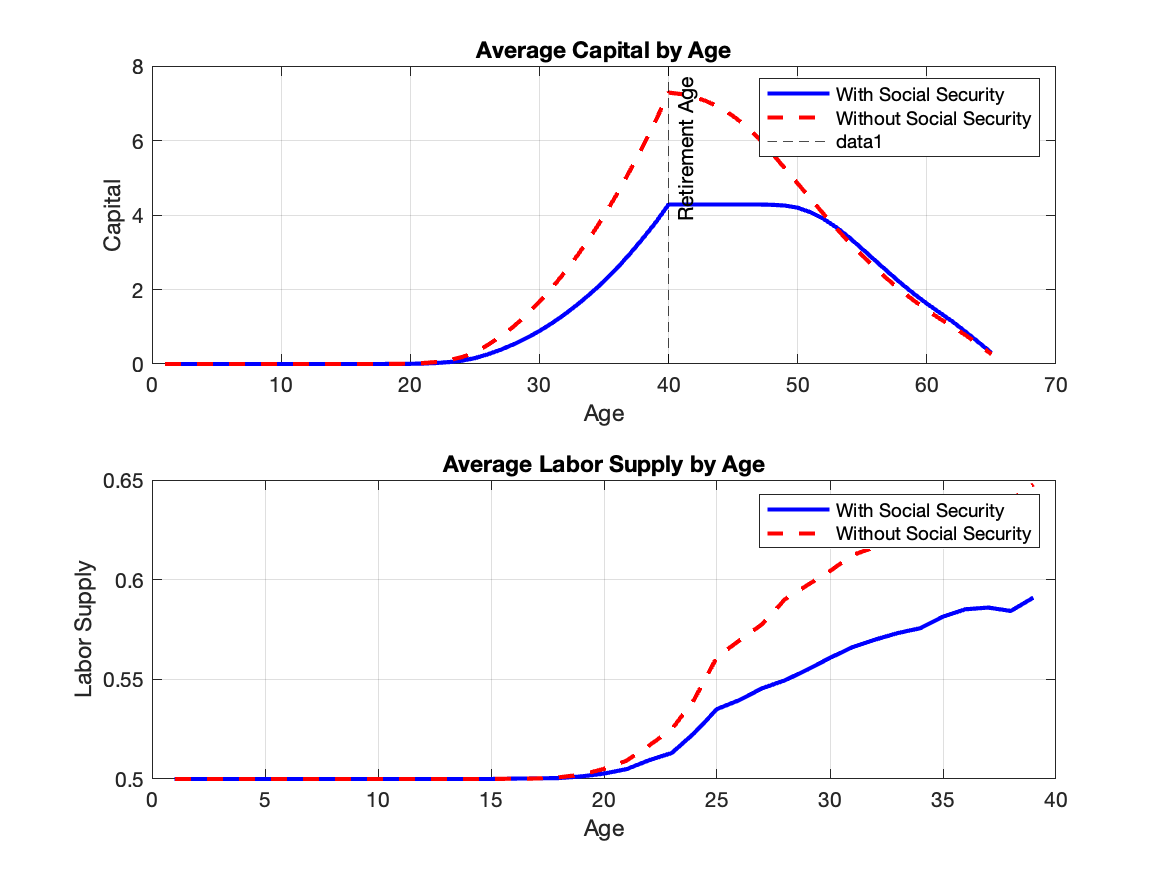
\includegraphics[width=\textwidth]{wealth_labor_profiles.png}

The wealth profile is higher without social security, as agents
hold more wealth without the taxation on their wages.
The labor supply profile is also higher without social security, as agents are incentivized to work more when they do not have to pay taxes on their wages.
\\

In the case where $\beta = 0.99$, the results of the policy experiment are as follows:


\begin{table}[h]
\centering
\begin{tabular}{|l|c|c|}
\hline
 & \multicolumn{2}{c|}{Benchmark model} \\
\cline{2-3}
 & with SS & without SS \\
\hline
capital $K$ & 2.6090 & 2.6092 \\
\hline
labor $L$ & 0.2320 & 0.2320 \\
\hline
wage $w$ & 1.5294 & 1.5295 \\
\hline
interest $r$ & 0.0166 & 0.0165 \\
\hline
pension benefit $b$ & \approx 0 & 0 \\
\hline
newborn welfare $V^o$ & -1705.4 & -1705.1 \\
\hline
\end{tabular}
\caption{Results of the policy experiment}
\end{table}

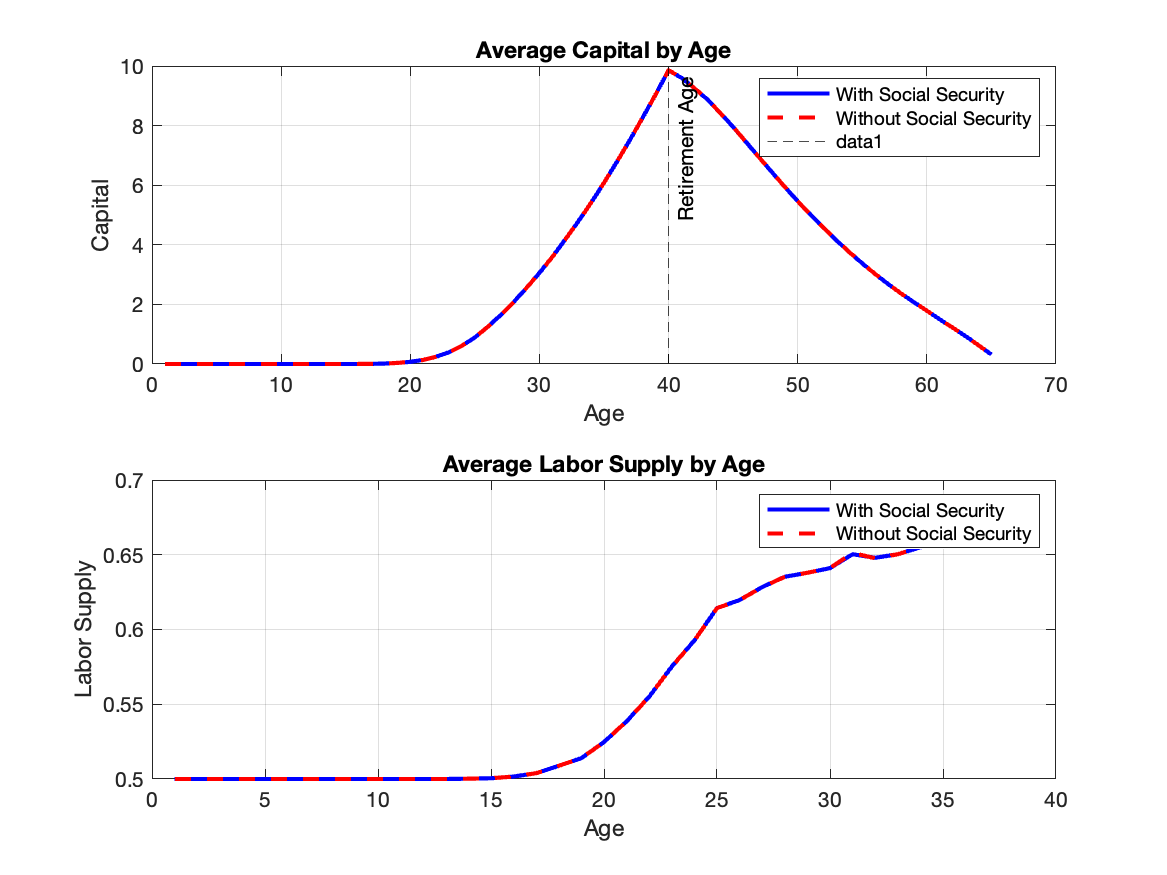
\includegraphics[width=\textwidth]{wealth_labor_profiles99.png}


In this case, Everything is practically the same, with slight differences due to rounding.
There is practically no difference in the capital, labor supply, and wage rates. Further, while
the case of no social security is still preferred, the difference in welfare is negligible.
\end{document}

